
\subsection{Approximate algorithms}

As it was explained in \label{sec1:subsec4} one of the main drawbacks of IDs
is the size of the decision tables to compute. Obviously this becomes a problem
when dealing with real-worlds IDs. In such kind of problems there are a lot of
variables in the modes and the sets of relevant variables for every decision
variable contain a lot of variables. And may happen that intermediate computations
require to compute even bigger potentials.

When this kind of IDs must be solved it is very important to have efficient
algorithms, focused on reducing the computational complexity, the storage requirements
and so on. Even for very complex IDs could be interesting to get approximate and
reduced solutions, even assumming that it is not exact at all. Such a solution
can offer some insight into the problem, perhaps during the construction of the
model, perhaps when the decision maker wants to confirm an overview of the
stretegy for a particular problem.

In Elvira two kind of approximate algorithms can be found:

\begin{itemize}
\item those using exact methods (arc reversal and variable elimination) and
taking advantage of the use of trees, as the one presented in \ref{prefTree}.

\item one based on simulation and focused on getting an approximation for
the solution but centered on the most probable combinations of values for the
variables of the model. This algorithm is specially devoted to complex
problems where a complete solution is unfeasible and the objective is to
know the course of action for the most common situations.
\end{itemize}

Both of these classes of algorithms will be explained below.

\subsubsection{Approximate algorithms using trees}

As it was mentioned before, all of these algorithms uses trees as an efficient
way to encode probabilities (\textit{probability trees}) and preferences 
(\textit{utility trees}). To get an unified notation for both kind of trees them 
will be termed \textit{numerical trees}. Here it will be explained how numerical
trees can be used to approximate computations and to deal with asymmetries (the
other main IDs drawback). As these algorithms are based on trees properties, we
begin making an overview on the operations that can be used to reduce the
computational complexity of IDs evaluation.

All the operations required to evaluate an ID can be directoly made on numerical
trees. In (ref 4 de numerical trees and ref 19 de numerical trees) this is
deeply explained, as well as a detailed explanation about how to build a numerical
tree from a given potential specified as a table of values. But to take advantage
of the hierarchical storage of information the trees offer another operations
are needed: sorting, pruning and approximation. With all of them trees can be
reduced, getting so a more compact an efficient representation. All of them are
briefly described below:

\begin{itemize}
\item \textit{Sorting}, rearranging the position of the variables and promoting
the most informative ones towards the root. This rearrangement tends to reduce
the differences between the values stored in the leafs, what facilitates the
later application of pruning and approximation operations.

\item \textit{Pruning}. This operation detects the proximity between the values
in the leafs of the tree, compressing them if possible: if the values are close
enough (under a given criteria) then all of them can be represented with only
one value derived from them. As it will be explained later, this operation is
specially relevant when it is combined with constraints. We will consider two
kind of pruning: exact and approximate, depending on the criteria of proximity
used.

\item \textit{Approximation} of the values stored in the trees. In fact this
operation is a combination of the previous ones, where the prune is done on
non-equal values (approximate pruning).
\end{itemize}

\subsubsection{Sorting numerical trees}

Sorting tries to reveals the most informative variables, preparing the tree
for posterior pruning operations. The key point here is to measure the
information that every variable adds to the tree. To explain this suppose
the tree to sort is $\mathcal{T}$, being $Z_{I}$ its domain. The initial ranking 
for the variables is achieved building a tree ${\cal T}'_X$ with only one of the 
variables $X \in Z_I$. In a leaf, say $x_i$, the value to store is $\sum {\cal T}(X=x_i,*)/card(\Omega_{Z_{I} \setminus X})$, where $*$ means the configurations 
in $\Omega_{Z_{I} \setminus X}$. The measure of information depends on the kind of 
potential. For probability potentials is the Kullback-Leibler cross entropy 
{cita 12 de numerical trees} between the original tree and the one with $X$ as root 
and no more variables:

\begin{equation}
\label{eq:KL}
D(\mathcal{T},\mathcal{T}'_X)=\sum_{ {\mathbf{z}}_{I} \in \Omega_{Z_I}}  \mathcal{T}(\mathbf{z}_I)\log
\frac{{\cal T}(\mathbf{z}_I)}{\mathcal{T}'_{X}(\mathbf{z}_I)}
\end{equation}

For utility trees the most informative variables will be those having more impact in 
the values of utility.  Here the measure is based on the Euclidean distance between 
the expected utility from both trees:

\begin{equation}
\label{eq:ED}
EUDiff(\mathcal{T},\mathcal{T}')=\sqrt{\sum_{\mathbf{z}_I\in \Omega{Z_I}} {(\mathcal{T}(\mathbf{z}_I) - \mathcal{T}'_{X} (\mathbf{z}_I))} ^2}
\end{equation}

But it turns out convenient to do an additional comment about utilities.  Suppose the utility 
tree in Fig. \ref{sortUtilities}(a), as well as the trees built to get the measure for $A$ 
(Fig. \ref{sortUtilities}(b)) and $D_2$ (Fig. \ref{sortUtilities}(c)). In the last two figures 
two equivalent representations of the same tree are shown; a summarized one (to the left) and 
another expanded (to the right).  The right ones are employed to show the matches between the 
original tree and the built ones (marked as $*$). Using \ref{eq:ED} the expected utility 
differences are $13.66, EUDiff({\cal T}, {\cal T}'_{A})$ and 
$16.57, EUDiff(\mathcal{T}, \mathcal{T}'_{D_2})$. Thus $A$ should be selected as the root of the tree. Nevertheless, if it is desired to obtain a more compact tree it is preferably D2 be the root 
variable. Observe that the tree used to measure $A$ information does not present matches respect 
to the original one while $D_2$ tree presents $6$ matches. This way, it turns out advisable to 
modify the measurement of distance previously considered, to include the proximity with respect 
to the original tree too. With this change is selected as root that variable having by itself a 
heavy weight in the utility (low Euclidean distance), but being able to offer a good approximation 
to the original values as well. The final distance can be computed like this:

\begin{equation}
\label{eq:EDMod}
D({\cal T},{\cal T}')=EUDiff({\cal T},{\cal T}') - EUDiff({\cal T},{\cal T}') * matches/size(\cal T)
\end{equation}

For 0 matches it is computed the Euclidean distance between the trees. However, as long as the 
number of matches is increased, there is a discount proportional to the proximity respect to the 
initial values. This will help posterior operations on the tree, as it will be shown later.

%Figuras de aproximaci�n de utilidades
\begin{figure*}[h]
\begin{center}
\begin{tabular}{c}
\subtable[Original tree]
{
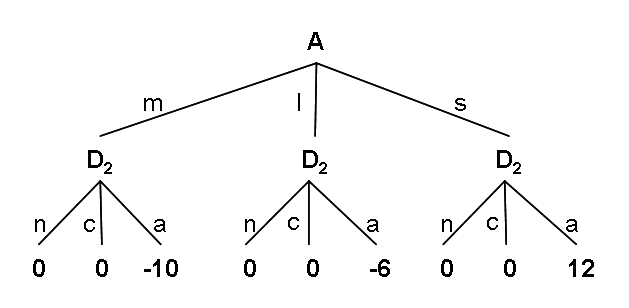
\includegraphics[scale=0.5]{./ID/fig/utilSort.eps}
} \\
\subtable[Information for $A$]
{
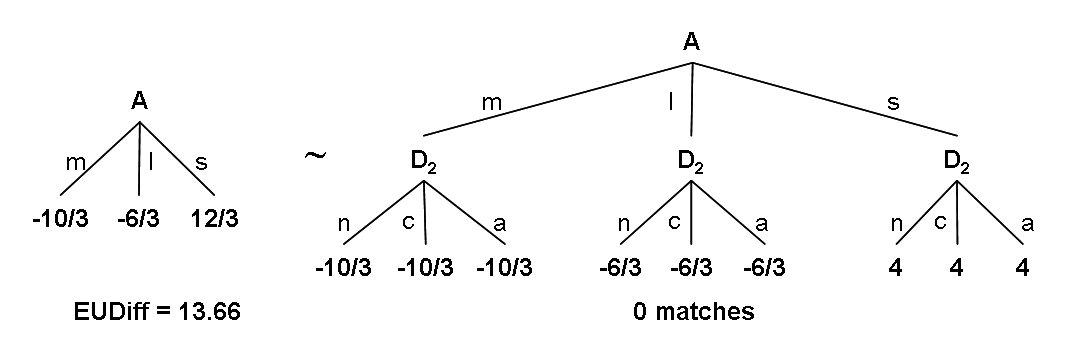
\includegraphics[scale=0.5]{./ID/fig/utilSortA.eps}
} \\
\subtable[Information for $D_2$]
{
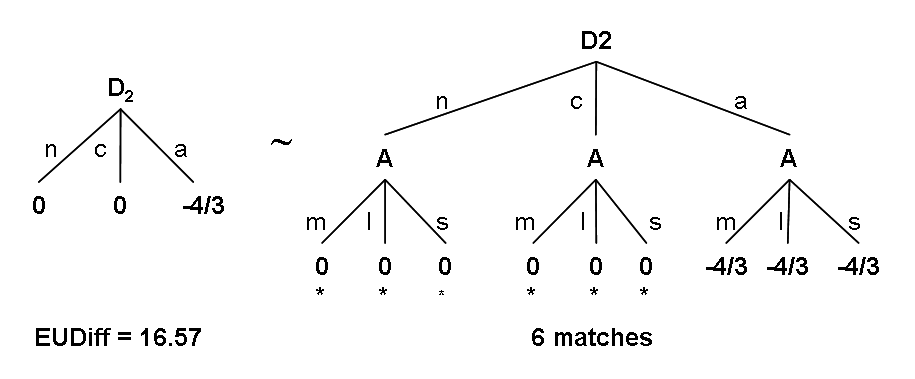
\includegraphics[scale=0.5]{./ID/fig/utilSortD2.eps}
} \\
\end{tabular}
\end{center}
\vspace{-0.7cm}
\caption{Sorting utility tree}
\label{sortUtilities}
\end{figure*}
%Fin de Figuras de aproximaci�n de utilidades

Once a variable has been added, the procedure is repeated, adding variables step
by step. The final utility tree after completing the sorting is presented in
Fig. \ref{utilSortFinal}.

\begin{figure*}[hbt]
\begin{center}
%%\resizebox{0.45\textwidth}{!}{\includegraphics{graficos/treeC2.eps}}
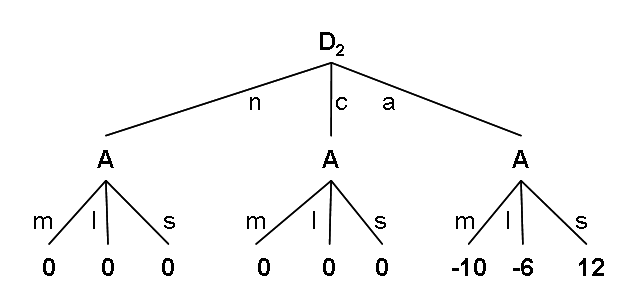
\includegraphics[scale=0.5]{./ID/fig/utilSortFinal.eps}
\end{center}
\vspace{-0.7cm}
\caption{Sorted utility tree for $\psi(D_2,A)$}
\label{utilSortFinal}
\end{figure*}


An example about sorting probability trees is shown below. Fig. 
\ref{treeprobtr} corresponds to the original tree and Fig. \ref{treeprobtrSorted}
shows the same tree after being sorted. It can be appreciated that $TR$ variable
is promoted till the root of the tree.

\begin{figure*}[hbt]
\begin{center}
%%\resizebox{1\textwidth}{!}{\includegraphics{graficos/treeprobtr.eps}}
\includegraphics[scale=0.5]{./ID/fig/treeprobtr.eps}
\end{center}
\vspace{-0.7cm}
\caption{Probability tree for $P(TR|D1, A)$}
\label{treeprobtr}
\end{figure*}

\begin{figure*}[hbt]
\begin{center}
%%\resizebox{0.45\textwidth}{!}{\includegraphics{graficos/treeC2.eps}}
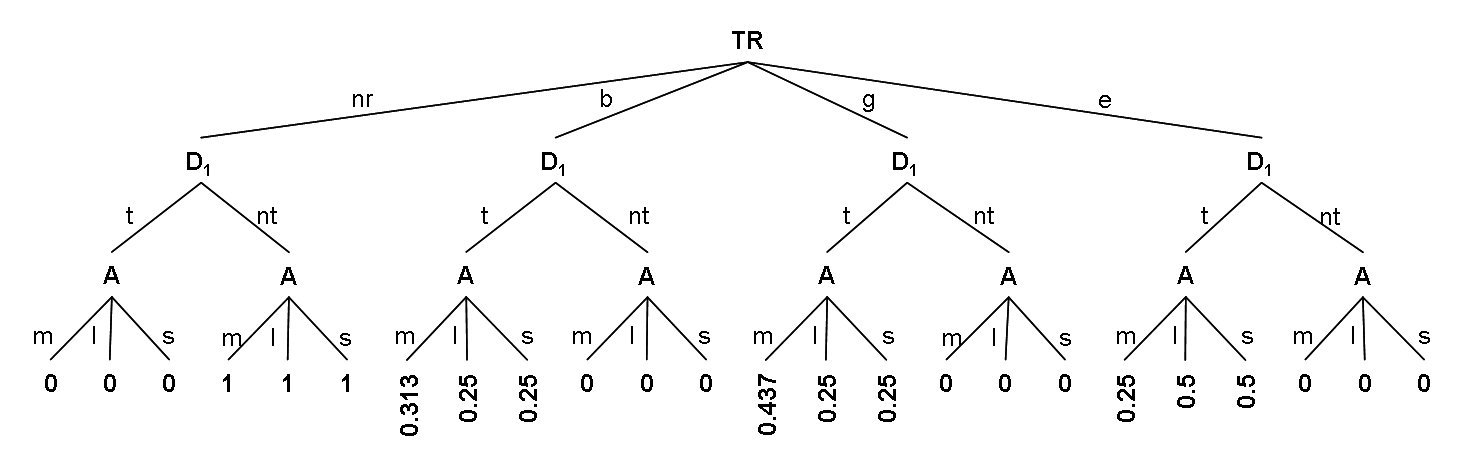
\includegraphics[scale=0.5]{./ID/fig/treeprobtrSorted.eps}
\end{center}
\vspace{-0.7cm}
\caption{Sorted tree for $P(TR|D_1,A)$}
\label{treeprobtrSorted}
\end{figure*}

\subsubsection{Pruning numerical trees}

The goal for this operation is to reduce trees as much as possible, taking advantage
of their hierarchical nature and avoiding the redundant storage of values. The leaf
nodes are examined and collapsed into a single value if they are close enough. To
make leave values be as close as possible, a sort operation it used to be done
previously. For example, taking into account the probability tree in Fig. 
\ref{treeprobSorted}, the pruning operation produces the reduced tree in Fig.
\ref{treeprobtrSortedPrunned}.

\begin{figure*}[hbt]
\begin{center}
%%\resizebox{0.45\textwidth}{!}{\includegraphics{graficos/treeC2.eps}}
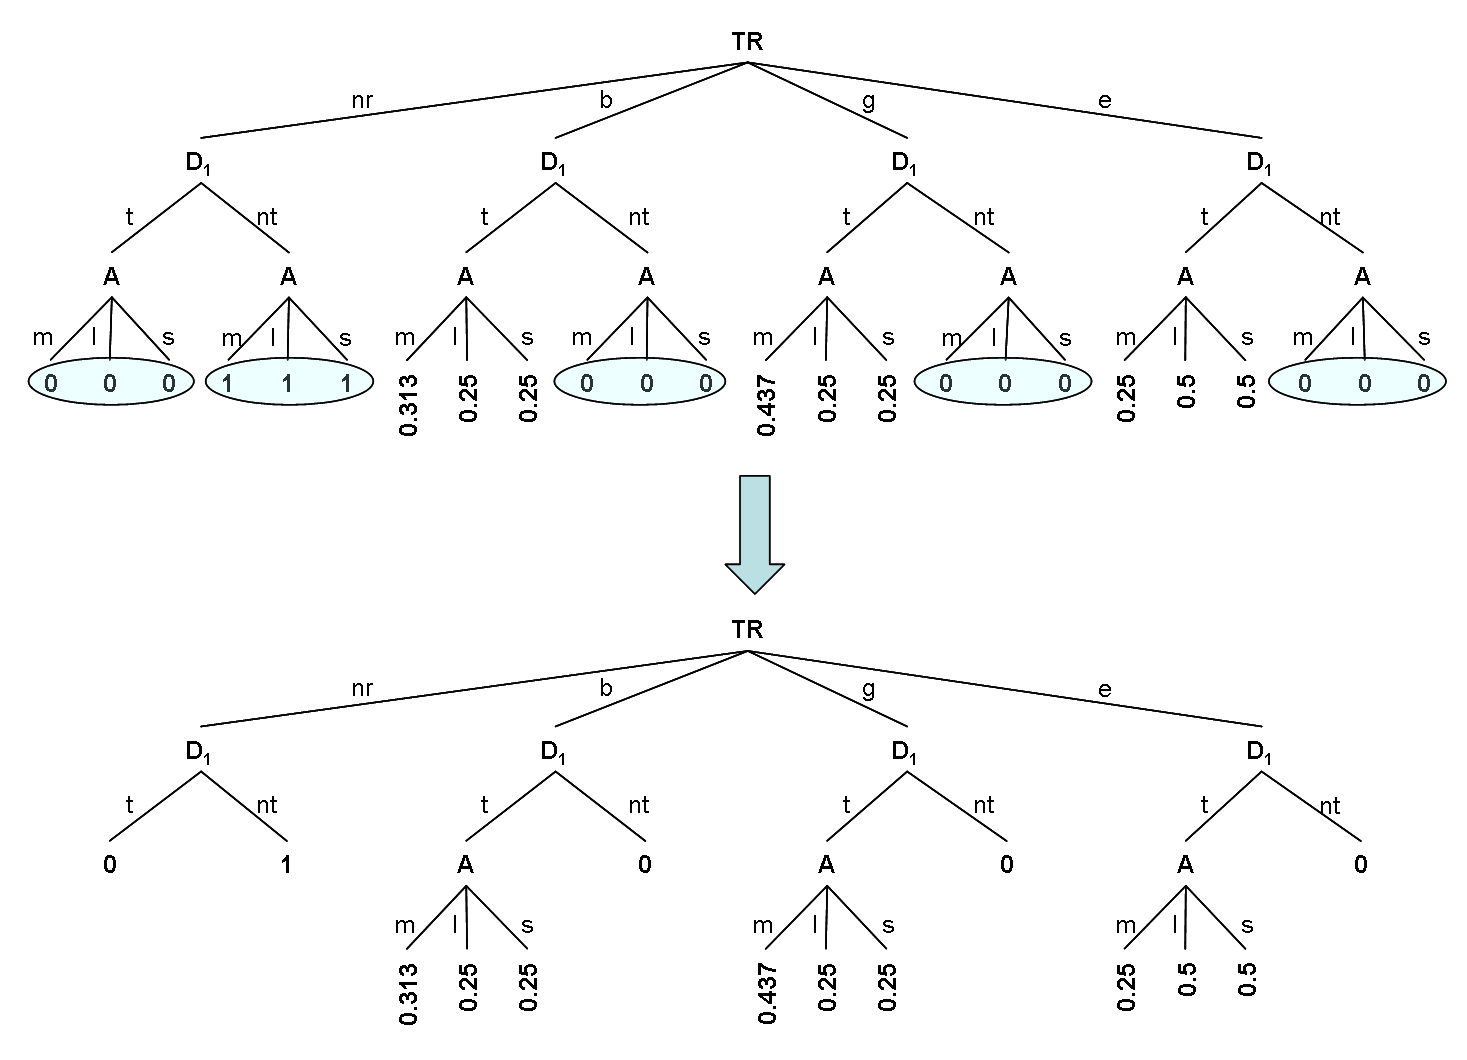
\includegraphics[scale=0.5]{./ID/fig/treeprobtrPrunned.eps}
\end{center}
\vspace{-0.7cm}
\caption{Sorted and pruned tree for $P(TR|D_1,A)$}
\label{treeprobtrSortedPrunned}
\end{figure*}

The same procedure can be applied on utility trees: observe the Fig. \ref{utilSortPrunned}.

\begin{figure*}[hbt]
\begin{center}
%%\resizebox{0.45\textwidth}{!}{\includegraphics{graficos/treeC2.eps}}
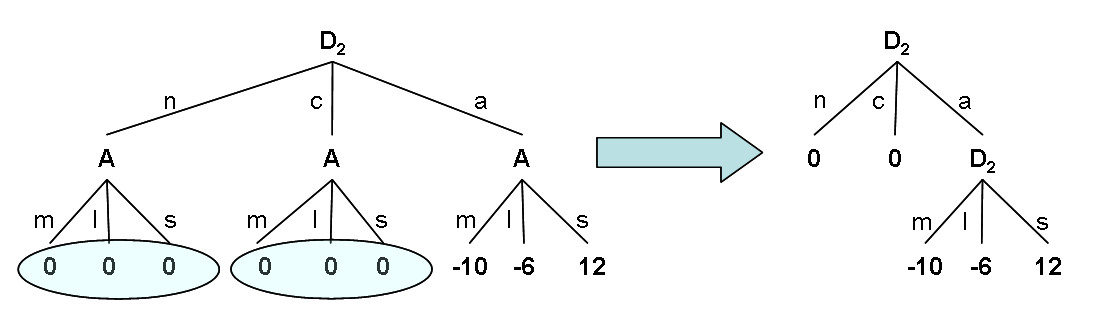
\includegraphics[scale=0.5]{./ID/fig/utilSortPrunned.eps}
\end{center}
\vspace{-0.7cm}
\caption{Sorted and pruned tree for $\psi(D_2,A)$}
\label{utilSortPrunned}
\end{figure*}

It must be observed that in this case the proximity criteria is the equality: several
values will be collapsed into one if them are exactly the same. The approximation
operation, explained below, relaxes this condition trying to reduce the trees as
much as possible, obviously assuming a lost of information.

\subsubsection{Approximating probability trees}

Pruning, sorting and approximation are closely related. In fact, the first two
are required to get an approximate tree from another one. The basic idea of the 
approximation is based on extending the exact pruning operation, so that not only 
identical values are collapsed, but also those that are near enough.  In general, 
the problem consists in approximating a numerical tree
$\mathcal{T}_{\phi}$ by another tree $\mathcal{T}'_{\phi}$ of a smaller size. For
probability trees, we will measure the {\em distance} between the
two potentials by the Kullback-Leibler cross entropy \cite{kule51} 
(see Eq. \ref{eq:KL}) between $\phi$ and $\phi'$. Therefore, to perform an 
approximation is required to define a threshold value $\Delta$. This threshold 
will be used during pruning operations. Bigger values for $\Delta$ lead to
more reduced trees (and obviously, the approximate tree will present a bigger
difference respect to the original one).

As an example, let us consider the probability tree presented in Fig. 
\ref{treeprobtrSortedPrunned}. For a certain value of $\Delta$ it could be approximated 
with the following tree (see Fig. \ref{treeprobtrApprox}). Observe the values 
$0.313$, $0.25$ and $0.25$ are changed to $0.271$. 

\begin{figure*}[hbt]
\begin{center}
%%\resizebox{0.45\textwidth}{!}{\includegraphics{graficos/treeC2.eps}}
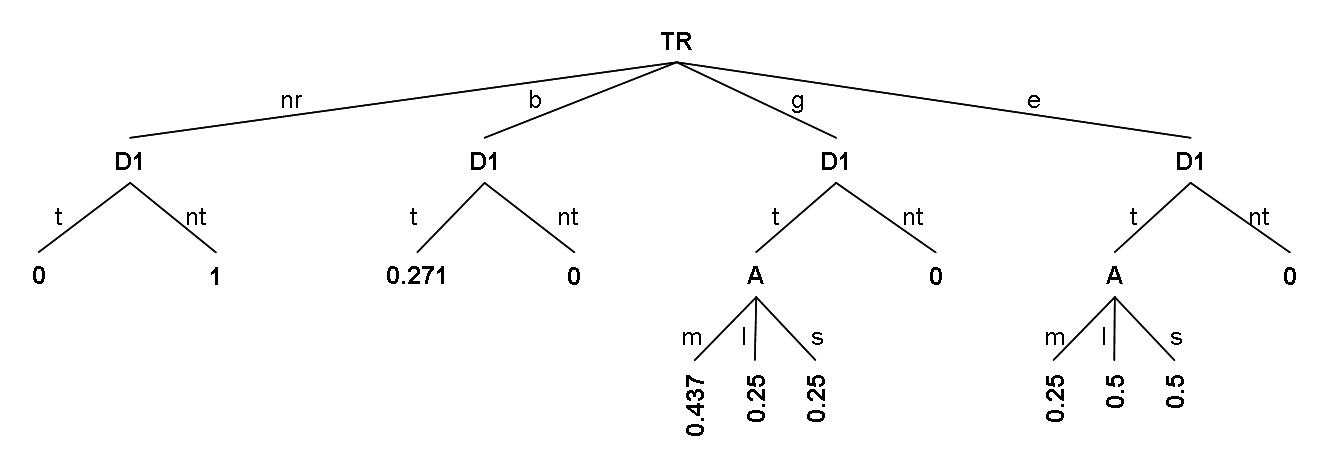
\includegraphics[scale=0.5]{./ID/fig/treeprobtrApprox.eps}
\end{center}
\vspace{-0.7cm}
\caption{Approximate tree for $P(TR|D_1,A)$}
\label{treeprobtrApprox}
\end{figure*}

\subsection{Applying constraints}

From a constraint rule we can obtain a numerical tree, a
\textit{constraint tree}. Constraint trees are used in the evaluation of
IDs in order to reduce the number of operations to perform and to assure 
that qualitative knowledge is considered.  Leaf nodes in constraint trees contain 
the values $0$ or $1$.  If $\mathcal{T}_{Z_{I}}$ is a constraint tree for the constraint 
rule $R(Z_I)$ defined on the set of variables $Z_I$, then a $0$ in a leaf node $\lambda$ 
means that the configuration leading to that node corresponds to an impossible 
scenario in the ID. A $1$ means that, taking into account only this constraint tree, 
the configuration is possible. For example, the constraint tree for the constraint included 
in \label{constraint} would be the one presented in Fig. \ref{constraintTree}.

\begin{figure*}[hbt]
\begin{center}
%%\resizebox{0.45\textwidth}{!}{\includegraphics{graficos/treeC2.eps}}
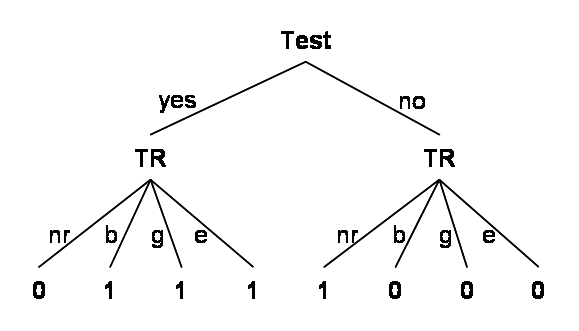
\includegraphics[scale=0.5]{./ID/fig/constraintTree.eps}
\end{center}
\vspace{-0.7cm}
\caption{Contraint tree}
\label{constraintTree}
\end{figure*}

In \ref{constraintTree} $TR$ means $TestResults$, being $nr$, $b$, $g$ and $e$ the
abbreviations for its states: $noResults$, $bad$, $good$ and $excellent$. During
the evaluation of an ID, when the variables related to a constraint belong to the
domain of a potential (with probabilities or utilities), both of them can be 
combined, ensuring the qualitative knowledge about the problem is considered. And,
as a second advantage, the combination of both potentials may facilitate the pruning
on the tree (all the leaves with 0 values can be collapsed).

Once these operations have been considered, it is easy to understand the way to
modify the algorithms previously described, arc reversal and variable elimination:

\begin{itemize}
\item First at all, trees are used to encode probabilities and utilities. If these
numerical data are contained in tables, it is needed to convert them into trees.
\item When a new tree is produced (as a conversion from a table or as a result
of combining or marginalizing, etc) its variables are sorted, making a posterior
pruning using the desired threshold for the aproximation. As it was mentioned
before, as long as the value of the threshold is increased, the final tree will
be farest from the initial one.
\end{itemize}

Making this, the final solution of the problem, is an approximation to the exact
one. The \textit{distance} between them it will depend on the threshold used for
the pruning operation and on the ID itself.


